% Chapter 26: Robustness and Uncertainty
% IEEE-formatted LaTeX chapter for Control Systems Textbook
% Self-contained chapter - can be \input{} into main document

\chapter{Robustness and Uncertainty}
\label{ch:robustness}

\begin{abstract}
This chapter develops the theory and practice of robust control---designing controllers that perform reliably despite inevitable discrepancies between mathematical models and physical reality. Beginning with Bode's foundational insights on sensitivity and progressing through the modern $H_\infty$ framework, we establish rigorous methods for quantifying and accommodating uncertainty. The practical laboratory demonstrates these principles through motor control with varying payloads, showing how robust design principles yield controllers that succeed where aggressive ``optimal'' designs fail.
\end{abstract}

%=============================================================================
\section{Historical Motivation: Why Models Are Never Enough}
\label{sec:robustness_history}
%=============================================================================

The history of control engineering is punctuated by spectacular failures---systems that worked perfectly in simulation yet failed catastrophically in deployment. These failures share a common root cause: the designer trusted the model too completely. Robust control theory emerged from the recognition that uncertainty is not an inconvenience to be minimized, but a fundamental reality to be embraced in the design process.

\subsection{Bode and the Origins of Robustness Thinking (1940s)}
\label{subsec:bode}

Hendrik Wade Bode, working at Bell Telephone Laboratories in the 1930s and 1940s, laid the conceptual foundation for robust control without ever using that term. His challenge was designing feedback amplifiers for transcontinental telephone transmission---systems that would operate continuously for decades across thousands of miles, through temperature extremes, component aging, and manufacturing variations.

\subsubsection{The Telephone Amplifier Problem}

A transcontinental telephone call in 1940 passed through dozens of repeater amplifiers, each boosting the signal to compensate for cable losses. The system faced fundamental uncertainties:

\begin{itemize}
    \item \textbf{Component drift}: Vacuum tube gains varied by 20--30\% over their lifetime
    \item \textbf{Temperature dependence}: Cables buried underground experienced seasonal temperature swings of 50°C or more, changing their attenuation characteristics
    \item \textbf{Manufacturing tolerances}: No two amplifiers were identical
    \item \textbf{Load variations}: The number of simultaneous calls affected impedance matching
\end{itemize}

An open-loop amplifier design was unthinkable---the cumulative gain variations would make the system unusable within months. Bode's insight was that feedback could be used not merely to improve nominal performance, but to \textit{desensitize} the system to parameter variations.

\subsubsection{The Sensitivity Function}

Bode formalized the concept of sensitivity in his 1945 book \textit{Network Analysis and Feedback Amplifier Design}. For a closed-loop system with loop transfer function $L(s)$, he defined the sensitivity function:
\begin{equation}
S(s) = \frac{1}{1 + L(s)}
\label{eq:sensitivity_bode}
\end{equation}

This function quantifies how much plant variations propagate to the closed-loop response. At frequencies where $|L(j\omega)| \gg 1$, we have $|S(j\omega)| \ll 1$, and the system is insensitive to plant variations. Bode recognized that this desensitization came at a cost---the complementary sensitivity function $T(s) = L(s)/(1+L(s))$ satisfies $S(s) + T(s) = 1$, implying that sensitivity reduction at one frequency range must be paid for elsewhere.

\subsubsection{Gain and Phase Margins}

Bode also introduced the concepts of gain margin and phase margin as practical robustness measures. Rather than asking ``Is the system stable?'' he asked ``How much can the system change before it becomes unstable?'' This shift in perspective---from binary stability to quantified robustness---was revolutionary.

\begin{definition}[Gain Margin]
The gain margin $G_m$ is the factor by which the loop gain can be multiplied before the system becomes unstable:
\begin{equation}
G_m = \frac{1}{|L(j\omega_\pi)|}
\label{eq:gain_margin}
\end{equation}
where $\omega_\pi$ is the frequency at which $\angle L(j\omega_\pi) = -180°$.
\end{definition}

\begin{definition}[Phase Margin]
The phase margin $\phi_m$ is the additional phase lag that would make the system marginally stable:
\begin{equation}
\phi_m = 180° + \angle L(j\omega_c)
\label{eq:phase_margin}
\end{equation}
where $\omega_c$ is the gain crossover frequency where $|L(j\omega_c)| = 1$.
\end{definition}

Bode's design philosophy was to ensure adequate margins---typically $G_m > 6$ dB and $\phi_m > 45°$---so that the system would remain stable despite the inevitable uncertainties in the telephone network.

\subsection{The Multivariable Challenge: Doyle and Stein (1981)}
\label{subsec:doyle_stein}

For decades, Bode's classical methods served engineers well. However, as control applications expanded to multivariable systems---aircraft with multiple control surfaces, chemical plants with interacting loops, flexible spacecraft---classical SISO (single-input, single-output) methods proved inadequate.

The modern era of robust control began with a seminal 1981 paper by John Doyle and Gunter Stein: ``Multivariable Feedback Design: Concepts for a Classical/Modern Synthesis.'' This paper addressed a crisis in control theory: the elegant state-space methods of the 1960s (LQR, LQG) produced controllers with excellent nominal performance but often terrible robustness.

\subsubsection{The LQG Robustness Problem}

Linear Quadratic Gaussian (LQG) control combines optimal state feedback (LQR) with optimal state estimation (Kalman filter). In theory, LQG should provide excellent performance. In practice, Doyle demonstrated that LQG controllers could have arbitrarily poor robustness margins---even zero gain margin.

The fundamental issue was that LQR and Kalman filtering were optimized separately, each assuming perfect knowledge of the other. LQR assumes perfect state knowledge; the Kalman filter assumes exact plant dynamics. When combined, the guarantees of each component evaporated.

\subsubsection{Loop Transfer Recovery}

Doyle and Stein proposed Loop Transfer Recovery (LTR) as a systematic method to recover robustness in LQG designs. The key insight was that full-state LQR feedback inherently provides excellent robustness (infinite gain margin, 60° phase margin for SISO systems), but this robustness is destroyed when an observer is added. LTR designs the observer to asymptotically recover the loop transfer function of the full-state feedback design.

This work established a crucial principle: \textbf{robustness must be explicitly designed in}, not assumed as a byproduct of optimal performance.

\subsection{$H_\infty$ Control: Zames and the Optimization of Robustness (1981)}
\label{subsec:zames}

George Zames, working at McGill University, proposed a radical reconceptualization of the control design problem. Rather than optimizing performance for a nominal plant (as in LQG), he proposed optimizing worst-case performance over a set of plants---a paradigm he called $H_\infty$ optimal control.

\subsubsection{The $H_\infty$ Norm}

The $H_\infty$ norm of a transfer function $G(s)$ is defined as:
\begin{equation}
\|G\|_\infty = \sup_{\omega \in \mathbb{R}} |G(j\omega)|
\label{eq:hinf_norm}
\end{equation}

For SISO systems, this is simply the peak magnitude of the frequency response. For MIMO systems, $|G(j\omega)|$ is replaced by the maximum singular value $\bar{\sigma}(G(j\omega))$.

The $H_\infty$ norm has a powerful interpretation: it equals the induced norm from $L_2$ input signals to $L_2$ output signals:
\begin{equation}
\|G\|_\infty = \sup_{u \neq 0} \frac{\|y\|_{L_2}}{\|u\|_{L_2}}
\label{eq:hinf_induced}
\end{equation}

This means the $H_\infty$ norm bounds the worst-case energy amplification from input to output.

\subsubsection{Robust Stability via Small Gain}

Zames's fundamental contribution was connecting the $H_\infty$ norm to robust stability through the \textbf{Small Gain Theorem}:

\begin{theorem}[Small Gain Theorem]
Consider a feedback interconnection of two stable systems $M(s)$ and $\Delta(s)$. The closed-loop system is stable for all stable $\Delta$ with $\|\Delta\|_\infty < 1/\gamma$ if and only if $\|M\|_\infty \leq \gamma$.
\end{theorem}

This theorem transforms robust stability into a norm minimization problem: find a controller that minimizes $\|M\|_\infty$, where $M$ is a transfer function from uncertainty inputs to uncertainty outputs. The smaller $\|M\|_\infty$, the larger the class of uncertainties the system can tolerate.

\subsection{Lessons from Failure: When Models Betray Us}
\label{subsec:failures}

The importance of robust design is most vividly illustrated by high-profile failures where nominal models proved fatally inadequate.

\subsubsection{Hubble Space Telescope (1990)}

The Hubble Space Telescope was launched in April 1990, intended to revolutionize astronomy with unprecedented resolution. Within weeks, astronomers realized the images were blurred---the primary mirror had been ground to the wrong shape.

The root cause was a flawed null corrector used to test the mirror during manufacturing. The corrector had a spacing error of 1.3 mm, causing the mirror to be ground with spherical aberration. The quality control system detected anomalies but dismissed them as calibration artifacts.

From a control perspective, the lesson is stark: the mirror fabrication was an open-loop process with inadequate feedback. The null corrector was trusted as ground truth, but it was wrong. A robust approach would have used multiple independent measurement systems, each capable of detecting the others' errors.

\subsubsection{Mars Polar Lander (1999)}

The Mars Polar Lander was lost during its descent to the Martian surface in December 1999. Post-failure analysis identified the most probable cause: the flight software interpreted vibrations from leg deployment as ground contact, shutting down the descent engines while the spacecraft was still 40 meters above the surface.

The landing algorithm was designed for nominal conditions---smooth descent, clean sensor signals. But the actual system experienced leg deployment transients that the designers had not anticipated. A robust design would have required confirmation from multiple sensors over a sustained period before declaring touchdown.

\subsubsection{Boeing 737 MAX (2018-2019)}

Two crashes of Boeing 737 MAX aircraft in 2018 and 2019, killing 346 people, were caused by the Maneuvering Characteristics Augmentation System (MCAS) repeatedly commanding nose-down trim based on a single angle-of-attack sensor. When that sensor failed or gave erroneous readings, MCAS drove the aircraft into unrecoverable dives.

The MCAS design violated fundamental robust design principles:
\begin{itemize}
    \item Single point of failure: one sensor controlled a critical system
    \item No uncertainty modeling: erroneous sensors were not considered in the design
    \item Inadequate authority limits: MCAS could command unlimited nose-down trim
    \item Pilot override inadequate: the system repeatedly reactivated after pilot correction
\end{itemize}

\subsection{The Fundamental Principle}
\label{subsec:fundamental}

These failures illuminate a principle that robust control theory formalizes mathematically:

\begin{tcolorbox}[colback=blue!5!white,colframe=blue!75!black,title=The Robustness Principle]
\textbf{All models are wrong.} A control system designed only for nominal conditions will fail when (not if) reality deviates from assumptions. Robust design explicitly accounts for uncertainty, ensuring acceptable performance across a range of operating conditions.
\end{tcolorbox}

The statistician George Box's famous aphorism---``All models are wrong, but some are useful''---takes on urgent meaning in control engineering. The question is not whether our model is perfect (it never is), but whether our controller can tolerate the model's imperfections.

%=============================================================================
\section{Modern Applications of Robust Control}
\label{sec:modern_applications}
%=============================================================================

Robust control principles find application wherever uncertainty is unavoidable and the consequences of failure are severe.

\subsection{Aerospace Systems}

Modern aircraft operate across vast flight envelopes where aerodynamic characteristics change dramatically:

\begin{itemize}
    \item \textbf{Mach number effects}: Transonic flight (Mach 0.8--1.2) exhibits complex shock-boundary layer interactions that defy precise modeling
    \item \textbf{Altitude variations}: Air density varies by orders of magnitude from sea level to cruise altitude, changing control effectiveness
    \item \textbf{Fuel consumption}: Aircraft mass can decrease by 40\% during long flights as fuel is consumed
    \item \textbf{Configuration changes}: Flaps, slats, landing gear, and store releases change the aircraft's dynamics
    \item \textbf{Icing and damage}: Ice accumulation or battle damage can dramatically alter aerodynamics
\end{itemize}

Flight control systems must provide stable, predictable handling qualities across this entire operating space. Robust control techniques---particularly $H_\infty$ and $\mu$-synthesis---are now standard tools in flight control design.

\subsection{Robotics and Automation}

Industrial robots face continuous uncertainty:

\begin{itemize}
    \item \textbf{Payload variations}: A robot arm might handle payloads from empty gripper to maximum capacity, changing effective inertia by factors of 10 or more
    \item \textbf{Wear and degradation}: Gearbox backlash, bearing wear, and cable stretching accumulate over millions of cycles
    \item \textbf{Friction variations}: Static and dynamic friction depend on temperature, lubrication, and contamination
    \item \textbf{Flexible dynamics}: High-speed robots excite structural resonances that depend on configuration
\end{itemize}

Robust controllers enable robots to maintain precision despite these variations, reducing the need for frequent recalibration.

\subsection{Power Systems and Renewable Energy}

Modern power grids face unprecedented uncertainty from renewable generation:

\begin{itemize}
    \item \textbf{Solar variability}: Cloud passages can change solar farm output by 50\% in minutes
    \item \textbf{Wind intermittency}: Wind power fluctuates on time scales from seconds (gusts) to seasons
    \item \textbf{Demand uncertainty}: Electric vehicle charging and smart appliances create unpredictable load patterns
    \item \textbf{Grid topology changes}: Lines are switched for maintenance, faults, and optimization
\end{itemize}

Grid frequency and voltage control must maintain stability despite these uncertainties, requiring robust control strategies at all levels from individual generators to system-wide coordination.

\subsection{Medical Devices}

Medical control systems face patient-to-patient variability and the ultimate consequences of failure:

\begin{itemize}
    \item \textbf{Drug delivery}: Patient metabolism varies by factors of 3--10; a dose appropriate for one patient may be dangerous for another
    \item \textbf{Artificial organs}: Blood pump controllers must accommodate varying vascular resistance, patient activity, and device degradation
    \item \textbf{Radiation therapy}: Tumor size and location change during treatment; beam control must adapt
\end{itemize}

Robust design is not optional in medical devices---it is the difference between healing and harm.

%=============================================================================
\section{Mathematical Foundations of Robust Control}
\label{sec:math_foundations}
%=============================================================================

We now develop the mathematical framework for analyzing and designing robust control systems.

\subsection{Types of Uncertainty}
\label{subsec:uncertainty_types}

Model uncertainty takes many forms, each requiring different mathematical treatment.

\subsubsection{Parametric Uncertainty}

Parametric uncertainty arises when the model structure is known but parameters are uncertain. Consider a DC motor with transfer function:
\begin{equation}
G(s) = \frac{K_m}{Js + B}
\label{eq:dc_motor}
\end{equation}
where $K_m$ is the motor constant, $J$ is the inertia, and $B$ is the viscous damping.

Each parameter lies in a known interval:
\begin{align}
K_m &\in [\underline{K}_m, \bar{K}_m] \\
J &\in [\underline{J}, \bar{J}] \\
B &\in [\underline{B}, \bar{B}]
\end{align}

The set of possible plants forms a ``box'' in parameter space. A robustly stable controller must stabilize all plants in this box.

\subsubsection{Unstructured Uncertainty}

Unstructured uncertainty represents unknown dynamics, typically at high frequencies where unmodeled resonances, nonlinearities, and time delays become significant. The key insight is that while we cannot specify these dynamics exactly, we can bound their magnitude as a function of frequency.

\begin{definition}[Unstructured Uncertainty Bound]
The unstructured uncertainty bound $W(s)$ is a transfer function such that the true plant $G_{\text{true}}(s)$ satisfies:
\begin{equation}
|G_{\text{true}}(j\omega) - G_{\text{nom}}(j\omega)| \leq |W(j\omega)|
\label{eq:unstructured_bound}
\end{equation}
for all frequencies $\omega$.
\end{definition}

This bound typically increases with frequency---at low frequencies, models are accurate; at high frequencies, unmodeled dynamics dominate.

\subsubsection{Additive Uncertainty}

In the additive uncertainty model, the true plant is expressed as:
\begin{equation}
G_{\text{true}}(s) = G_{\text{nom}}(s) + \Delta_a(s)
\label{eq:additive}
\end{equation}
where $\Delta_a(s)$ is stable and satisfies $\|\Delta_a\|_\infty < \|W_a\|_\infty$.

\begin{figure}[htbp]
\centering
\begin{tikzpicture}[auto, node distance=2.5cm, >=latex']
    % Blocks
    \node [input] (input) {};
    \node [block, right of=input] (gnom) {$G_{\text{nom}}(s)$};
    \node [sum, right of=gnom, node distance=2.5cm] (sum) {};
    \node [output, right of=sum, node distance=1.5cm] (output) {};

    % Uncertainty path
    \node [block, above of=gnom, node distance=1.5cm] (delta) {$\Delta_a(s)$};

    % Connections
    \draw [->] (input) -- node {$u$} (gnom);
    \draw [->] (gnom) -- node {} (sum);
    \draw [->] (sum) -- node {$y$} (output);

    % Uncertainty connection
    \draw [->] (input) |- (delta);
    \draw [->] (delta) -| (sum);

    % Sum labels
    \node at (sum.north) {$+$};
    \node at (sum.south west) {$+$};
\end{tikzpicture}
\caption{Additive uncertainty model: $G_{\text{true}} = G_{\text{nom}} + \Delta_a$}
\label{fig:additive}
\end{figure}

\subsubsection{Multiplicative Uncertainty}

The multiplicative uncertainty model is often more natural for physical systems:
\begin{equation}
G_{\text{true}}(s) = G_{\text{nom}}(s)(1 + \Delta_m(s) W_m(s))
\label{eq:multiplicative}
\end{equation}
where $\|\Delta_m\|_\infty < 1$ and $W_m(s)$ is the uncertainty weight.

The multiplicative form has a clear interpretation: $|W_m(j\omega)|$ represents the fractional uncertainty at frequency $\omega$. If $|W_m(j\omega)| = 0.2$ at some frequency, the plant gain at that frequency is uncertain by $\pm 20\%$.

\begin{figure}[htbp]
\centering
\begin{tikzpicture}[auto, node distance=2cm, >=latex']
    % Main path
    \node [input] (input) {};
    \node [block, right of=input, node distance=2.5cm] (gnom) {$G_{\text{nom}}(s)$};
    \node [sum, right of=gnom, node distance=2.5cm] (sum) {};
    \node [output, right of=sum, node distance=1.5cm] (output) {};

    % Uncertainty path
    \node [block, above of=gnom, node distance=1.5cm, minimum width=2em] (wm) {$W_m$};
    \node [block, right of=wm, node distance=2cm, minimum width=2em] (delta) {$\Delta_m$};

    % Connections
    \draw [->] (input) -- node {$u$} (gnom);
    \draw [->] (gnom) -- (sum);
    \draw [->] (sum) -- node {$y$} (output);

    % Uncertainty connections
    \draw [->] (input) |- (wm);
    \draw [->] (wm) -- (delta);
    \draw [->] (delta) -| (sum);

    \node at (sum.north) {$+$};
    \node at (sum.south west) {$+$};
\end{tikzpicture}
\caption{Multiplicative uncertainty model: $G_{\text{true}} = G_{\text{nom}}(1 + W_m\Delta_m)$}
\label{fig:multiplicative}
\end{figure}

\subsubsection{Input and Output Multiplicative Uncertainty}

For multivariable systems, we distinguish:
\begin{align}
G_{\text{true}}(s) &= (I + \Delta_o W_o) G_{\text{nom}}(s) && \text{(output multiplicative)} \\
G_{\text{true}}(s) &= G_{\text{nom}}(s) (I + W_i \Delta_i) && \text{(input multiplicative)}
\end{align}

Output multiplicative uncertainty is appropriate when the uncertainty affects sensor measurements or output channels. Input multiplicative uncertainty models actuator variations.

\subsection{The Small Gain Theorem}
\label{subsec:small_gain}

The Small Gain Theorem is the cornerstone of robust stability analysis. Consider a feedback interconnection of two systems $M(s)$ and $\Delta(s)$:

\begin{figure}[htbp]
\centering
\begin{tikzpicture}[auto, node distance=2.5cm, >=latex']
    \node [block, minimum width=3em, minimum height=2em] (M) {$M(s)$};
    \node [block, below of=M, node distance=2cm, minimum width=3em, minimum height=2em] (Delta) {$\Delta(s)$};

    % Connections
    \draw [->] (M.east) -- ++(0.8,0) |- (Delta.east);
    \draw [->] (Delta.west) -- ++(-0.8,0) |- (M.west);

    % Labels
    \node [right of=M, node distance=1.5cm] {$z$};
    \node [left of=M, node distance=1.5cm] {$w$};
\end{tikzpicture}
\caption{Standard feedback interconnection for Small Gain Theorem}
\label{fig:small_gain}
\end{figure}

\begin{theorem}[Small Gain Theorem]
\label{thm:small_gain}
Assume $M(s)$ is stable and $\Delta(s)$ is stable with $\|\Delta\|_\infty \leq 1$. Then the feedback interconnection is stable if:
\begin{equation}
\|M\|_\infty < 1
\label{eq:small_gain}
\end{equation}
\end{theorem}

\begin{proof}
Consider the closed-loop equations:
\begin{align}
z &= M w \\
w &= \Delta z
\end{align}

Taking $L_2$ norms:
\begin{align}
\|z\|_{L_2} &\leq \|M\|_\infty \|w\|_{L_2} \\
\|w\|_{L_2} &\leq \|\Delta\|_\infty \|z\|_{L_2}
\end{align}

Substituting:
\begin{equation}
\|z\|_{L_2} \leq \|M\|_\infty \|\Delta\|_\infty \|z\|_{L_2}
\end{equation}

If $\|M\|_\infty \|\Delta\|_\infty < 1$, this implies $\|z\|_{L_2}$ is finite for any finite input, hence the system is stable.
\end{proof}

\subsubsection{Interpretation for Robust Stability}

For a control system with multiplicative uncertainty, the relevant transfer function $M(s)$ is the complementary sensitivity function $T(s)$:

\begin{theorem}[Robust Stability with Multiplicative Uncertainty]
\label{thm:robust_stab_mult}
Consider a feedback system with plant $G_{\text{true}} = G_{\text{nom}}(1 + W_m\Delta_m)$, $\|\Delta_m\|_\infty \leq 1$, and controller $K(s)$. The closed-loop system is robustly stable if and only if:
\begin{equation}
\|W_m T\|_\infty < 1
\label{eq:robust_stab_mult}
\end{equation}
where $T = \dfrac{G_{\text{nom}} K}{1 + G_{\text{nom}} K}$ is the nominal complementary sensitivity.
\end{theorem}

This result has a beautiful frequency-domain interpretation: at each frequency, we require:
\begin{equation}
|W_m(j\omega)| \cdot |T(j\omega)| < 1
\end{equation}

Where the uncertainty is large ($|W_m|$ large, typically at high frequencies), the complementary sensitivity $|T|$ must be small. Where the uncertainty is small, $|T|$ can be larger.

\subsection{Sensitivity Functions and Trade-offs}
\label{subsec:sensitivity}

The sensitivity function $S(s)$ and complementary sensitivity function $T(s)$ are the fundamental quantities in robust control:
\begin{align}
S(s) &= \frac{1}{1 + L(s)} \\
T(s) &= \frac{L(s)}{1 + L(s)}
\end{align}
where $L(s) = G(s)K(s)$ is the loop transfer function.

These functions satisfy the fundamental algebraic constraint:
\begin{equation}
S(s) + T(s) = 1
\label{eq:ST_identity}
\end{equation}

\subsubsection{Frequency-Domain Shaping Requirements}

Good control requires:
\begin{itemize}
    \item \textbf{Low-frequency $|S|$ small}: For tracking and disturbance rejection, we want $|S(j\omega)| \ll 1$ at low frequencies. This requires $|L(j\omega)| \gg 1$.
    \item \textbf{High-frequency $|T|$ small}: For noise rejection and robustness to unmodeled dynamics, we want $|T(j\omega)| \ll 1$ at high frequencies. This requires $|L(j\omega)| \ll 1$.
\end{itemize}

The identity $S + T = 1$ shows that we cannot have both small simultaneously. At any frequency, either $|S|$ is small or $|T|$ is small, but not both.

\begin{figure}[htbp]
\centering
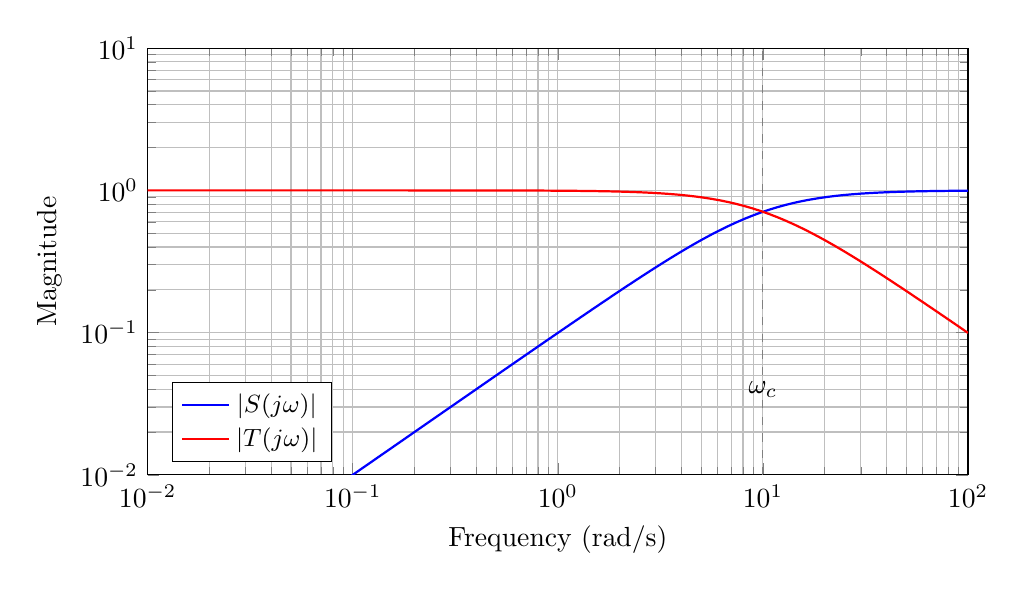
\begin{tikzpicture}
\begin{semilogyaxis}[
    width=12cm, height=7cm,
    xlabel={Frequency (rad/s)},
    ylabel={Magnitude},
    xmin=0.01, xmax=100,
    ymin=0.01, ymax=10,
    xmode=log,
    grid=both,
    legend pos=south west,
    legend style={font=\small}
]
% Sensitivity function
\addplot[blue, thick, domain=0.01:100, samples=100]
    {1/sqrt(1 + (10/x)^2)};
\addlegendentry{$|S(j\omega)|$}

% Complementary sensitivity
\addplot[red, thick, domain=0.01:100, samples=100]
    {(10/x)/sqrt(1 + (10/x)^2)};
\addlegendentry{$|T(j\omega)|$}

% Crossover
\addplot[dashed, gray] coordinates {(10, 0.01) (10, 10)};
\node at (axis cs:10, 0.03) [anchor=south] {$\omega_c$};

\end{semilogyaxis}
\end{tikzpicture}
\caption{Typical sensitivity and complementary sensitivity functions. At low frequencies, $|S|$ is small (good tracking). At high frequencies, $|T|$ is small (robustness). The crossover frequency $\omega_c$ marks the transition.}
\label{fig:ST_bode}
\end{figure}

\subsubsection{Sensitivity Peaks and Robustness}

The peak values of $S$ and $T$ are key robustness indicators:
\begin{align}
M_S &= \|S\|_\infty = \max_\omega |S(j\omega)| \\
M_T &= \|T\|_\infty = \max_\omega |T(j\omega)|
\end{align}

The sensitivity peak $M_S$ is related to stability margins:
\begin{equation}
M_S = \frac{1}{\min_\omega |1 + L(j\omega)|} = \frac{1}{\text{distance from } -1 \text{ to Nyquist curve}}
\label{eq:MS_margin}
\end{equation}

\begin{theorem}[Margins from Sensitivity Peak]
\label{thm:margins_MS}
If $M_S$ is the peak sensitivity, then:
\begin{align}
\text{Gain margin:} \quad G_m &\geq \frac{M_S}{M_S - 1} \\
\text{Phase margin:} \quad \phi_m &\geq 2 \sin^{-1}\left(\frac{1}{2M_S}\right)
\end{align}
\end{theorem}

For example, $M_S = 2$ (6 dB) guarantees $G_m \geq 2$ (6 dB) and $\phi_m \geq 29°$.

Recommended design specifications for robust systems:
\begin{itemize}
    \item $M_S \leq 2$ (6 dB) for good robustness
    \item $M_S \leq 1.5$ (3.5 dB) for critical applications
    \item $M_T \leq 1.25$ (2 dB) for robustness to multiplicative uncertainty
\end{itemize}

\subsection{The $H_\infty$ Control Problem}
\label{subsec:hinf_problem}

The $H_\infty$ control problem formalizes robust design as an optimization problem.

\subsubsection{Mixed Sensitivity Formulation}

The mixed sensitivity problem seeks a controller $K(s)$ that minimizes:
\begin{equation}
\left\| \begin{bmatrix} W_S S \\ W_T T \end{bmatrix} \right\|_\infty
\label{eq:mixed_sensitivity}
\end{equation}
where $W_S(s)$ and $W_T(s)$ are weighting functions.

This formulation simultaneously shapes both sensitivity functions:
\begin{itemize}
    \item $W_S$ is large at low frequencies, forcing $|S|$ small there (good tracking)
    \item $W_T$ is large at high frequencies, forcing $|T|$ small there (robustness)
\end{itemize}

\subsubsection{Standard Problem Formulation}

The general $H_\infty$ problem uses the ``standard plant'' formulation:

\begin{figure}[htbp]
\centering
\begin{tikzpicture}[auto, node distance=2.5cm, >=latex']
    \node [block, minimum width=4em, minimum height=4em] (P) {$P(s)$};
    \node [block, below of=P, node distance=2.5cm, minimum width=3em] (K) {$K(s)$};

    % External inputs/outputs
    \node [left of=P, node distance=2.5cm] (w) {$w$};
    \node [right of=P, node distance=2.5cm] (z) {$z$};

    % Control connections
    \draw [->] (w) -- (P);
    \draw [->] (P) -- (z);

    % Lower connections
    \coordinate [below left of=P, node distance=1.2cm] (y_in);
    \coordinate [below right of=P, node distance=1.2cm] (u_out);

    \draw [->] (P.south west) -- ++(-0.5,-0.5) -| (K.west);
    \draw [->] (K.east) -| ++(0.5,0.5) -- (P.south east);

    \node at ($(P.south west) + (-0.8,-0.3)$) {$y$};
    \node at ($(P.south east) + (0.8,-0.3)$) {$u$};
\end{tikzpicture}
\caption{Standard $H_\infty$ configuration}
\label{fig:hinf_standard}
\end{figure}

The generalized plant $P(s)$ is partitioned as:
\begin{equation}
\begin{bmatrix} z \\ y \end{bmatrix} = \begin{bmatrix} P_{11} & P_{12} \\ P_{21} & P_{22} \end{bmatrix} \begin{bmatrix} w \\ u \end{bmatrix}
\end{equation}

The closed-loop transfer function from $w$ to $z$ is:
\begin{equation}
T_{zw} = P_{11} + P_{12} K (I - P_{22} K)^{-1} P_{21} \triangleq \mathcal{F}_l(P, K)
\label{eq:lft}
\end{equation}

The $H_\infty$ optimal control problem is:
\begin{equation}
\min_K \| \mathcal{F}_l(P, K) \|_\infty \quad \text{subject to internal stability}
\end{equation}

\subsubsection{State-Space Solution}

For state-space plants, the $H_\infty$ problem can be solved via two algebraic Riccati equations. Given:
\begin{equation}
P(s) = \begin{bmatrix} A & B_1 & B_2 \\ \hline C_1 & D_{11} & D_{12} \\ C_2 & D_{21} & D_{22} \end{bmatrix}
\end{equation}

Under standard assumptions (including $D_{11} = 0$, $D_{22} = 0$), a stabilizing controller achieving $\|T_{zw}\|_\infty < \gamma$ exists if and only if:
\begin{enumerate}
    \item The $H_\infty$ control Riccati equation has a stabilizing solution $X_\infty \geq 0$
    \item The $H_\infty$ filtering Riccati equation has a stabilizing solution $Y_\infty \geq 0$
    \item The spectral radius condition $\rho(X_\infty Y_\infty) < \gamma^2$ holds
\end{enumerate}

The optimal $\gamma$ is found by bisection, and the controller is given by:
\begin{equation}
K(s) = \begin{bmatrix} A_K & B_K \\ \hline C_K & 0 \end{bmatrix}
\end{equation}
where the controller matrices depend on $X_\infty$, $Y_\infty$, and $\gamma$.

\subsection{Robust Performance}
\label{subsec:robust_perf}

Robust stability ensures the system remains stable for all plants in the uncertainty set. Robust performance goes further, requiring that performance specifications are met for all plants.

\subsubsection{Performance Weights}

Let $W_P(s)$ be a performance weight such that acceptable performance requires:
\begin{equation}
|W_P(j\omega) S(j\omega)| < 1 \quad \forall \omega
\end{equation}

This is equivalent to $\|W_P S\|_\infty < 1$.

\subsubsection{Combined Robust Stability and Robust Performance}

For multiplicative uncertainty with weight $W_m$ and performance weight $W_P$, the robust performance condition is:
\begin{equation}
\|W_P S\|_\infty + \|W_m T\|_\infty < 1
\label{eq:robust_perf_approx}
\end{equation}

A more precise condition uses the structured singular value ($\mu$), but (\ref{eq:robust_perf_approx}) provides a useful sufficient condition.

\subsection{Introduction to $\mu$-Analysis}
\label{subsec:mu}

When uncertainty has known structure (e.g., separate uncertainties in different parameters), the Small Gain Theorem can be conservative. The structured singular value $\mu$ provides tighter bounds.

\begin{definition}[Structured Singular Value]
For a complex matrix $M$ and a structured uncertainty set $\Delta$:
\begin{equation}
\mu_\Delta(M) = \frac{1}{\min\{\bar{\sigma}(\Delta) : \Delta \in \Delta, \det(I - M\Delta) = 0\}}
\label{eq:mu_def}
\end{equation}
\end{definition}

Robust stability holds for all $\Delta$ with $\bar{\sigma}(\Delta) < 1$ if and only if $\mu_\Delta(M) < 1$.

Computing $\mu$ exactly is NP-hard for general structures, but efficient algorithms provide tight upper and lower bounds. For purely real uncertainties (parametric), special techniques apply.

\subsection{Practical Robustness Assessment}
\label{subsec:practical}

While $H_\infty$ and $\mu$ provide rigorous frameworks, practical robustness assessment often uses simpler methods.

\subsubsection{Gain and Phase Margin Assessment}

For SISO systems, classical margins remain valuable:
\begin{itemize}
    \item Gain margin $G_m \geq 6$ dB (factor of 2)
    \item Phase margin $\phi_m \geq 45°$
    \item Delay margin $\tau_m = \phi_m/\omega_c$ (at least one sampling period for digital systems)
\end{itemize}

\subsubsection{Sensitivity Peak Limits}

Specify bounds on $M_S$ and $M_T$:
\begin{itemize}
    \item $M_S \leq 2$ (6 dB)
    \item $M_T \leq 1.25$ (2 dB)
\end{itemize}

\subsubsection{Monte Carlo Analysis}

For complex systems, simulate performance over random samples from the uncertainty set:
\begin{enumerate}
    \item Define probability distributions for uncertain parameters
    \item Generate $N$ random plant instances
    \item Simulate closed-loop response for each
    \item Compute statistics of performance metrics
    \item Identify worst-case scenarios
\end{enumerate}

This approach captures nonlinear effects and correlations that analytical methods may miss.

\subsubsection{Worst-Case Analysis}

Grid the uncertainty space and evaluate performance at each vertex (for parametric uncertainty) or at extremes (for unstructured uncertainty). This guarantees that the worst case within the grid is identified.

%=============================================================================
\section{Practical Laboratory: Robust Motor Control}
\label{sec:lab}
%=============================================================================

This laboratory demonstrates robust control principles using a DC motor with uncertain payload. Students will design both aggressive and conservative controllers, then test their performance as the payload varies.

\subsection{Learning Objectives}

Upon completion of this laboratory, students will be able to:
\begin{enumerate}
    \item Characterize plant uncertainty by measuring transfer function variations
    \item Design controllers for specified gain and phase margins
    \item Demonstrate the failure of aggressive controllers under perturbation
    \item Verify that robust controllers maintain stability across the uncertainty range
    \item Trade off performance versus robustness quantitatively
\end{enumerate}

\subsection{Required Components}

\begin{table}[htbp]
\centering
\caption{Bill of Materials for Robust Control Laboratory}
\label{tab:robust_bom}
\begin{tabular}{|l|l|l|}
\hline
\textbf{Component} & \textbf{Specification} & \textbf{Qty} \\
\hline
Arduino Uno/Nano & ATmega328P & 1 \\
DC Motor with Encoder & 12V, 400+ PPR & 1 \\
Motor Driver & L298N or TB6612 & 1 \\
Power Supply & 12V, 3A & 1 \\
Payload Masses & 10g, 25g, 50g, 100g & 4 \\
Mounting Hardware & 3D-printed wheel/arm & 1 \\
Breadboard \& Wires & Standard & 1 set \\
\hline
\end{tabular}
\end{table}

The key addition is the set of masses that attach to the motor shaft, simulating varying payload inertia.

\subsection{System Identification}

Before designing controllers, students characterize the plant with different payloads.

\subsubsection{Step Response Method}

Apply a step voltage to the motor and measure the velocity response. For a first-order approximation:
\begin{equation}
G(s) = \frac{K}{Js + B} = \frac{K/B}{(J/B)s + 1} = \frac{K_{\text{DC}}}{\tau s + 1}
\end{equation}

Measure:
\begin{itemize}
    \item Steady-state velocity $\omega_{ss} = K_{\text{DC}} \cdot V_{in}$
    \item Time constant $\tau$ = time to reach 63\% of steady-state
\end{itemize}

\begin{lstlisting}[language=C++, caption={System Identification Code}, label={lst:sysid}]
// System identification: step response
const int MOTOR_PWM = 5;
const int ENCODER_A = 2;
const int ENCODER_B = 3;

volatile long encoderCount = 0;
unsigned long startTime;
float lastVelocity = 0;
float velocities[500];  // Store velocity samples
unsigned long times[500];
int sampleIndex = 0;

void setup() {
    Serial.begin(115200);
    pinMode(MOTOR_PWM, OUTPUT);
    pinMode(ENCODER_A, INPUT_PULLUP);
    pinMode(ENCODER_B, INPUT_PULLUP);
    attachInterrupt(digitalPinToInterrupt(ENCODER_A),
                    encoderISR, RISING);

    Serial.println("System Identification");
    Serial.println("Applying step input in 2 seconds...");
    delay(2000);

    // Apply step
    startTime = millis();
    analogWrite(MOTOR_PWM, 150);  // 59% duty cycle
}

void loop() {
    static unsigned long lastSample = 0;
    unsigned long now = millis();

    // Sample at 100 Hz for 5 seconds
    if (now - lastSample >= 10 && sampleIndex < 500) {
        float velocity = getVelocity();  // deg/s
        velocities[sampleIndex] = velocity;
        times[sampleIndex] = now - startTime;
        sampleIndex++;
        lastSample = now;
    }

    // After 5 seconds, stop and print data
    if (now - startTime > 5000 && sampleIndex >= 500) {
        analogWrite(MOTOR_PWM, 0);
        Serial.println("Time(ms), Velocity(deg/s)");
        for (int i = 0; i < 500; i++) {
            Serial.print(times[i]);
            Serial.print(", ");
            Serial.println(velocities[i]);
        }
        while(1);  // Stop
    }
}

void encoderISR() {
    if (digitalRead(ENCODER_B)) encoderCount++;
    else encoderCount--;
}

float getVelocity() {
    static long lastCount = 0;
    static unsigned long lastTime = 0;
    unsigned long now = micros();
    long count = encoderCount;

    float dt = (now - lastTime) / 1.0e6;  // seconds
    float dTheta = (count - lastCount) * (360.0 / 400.0);  // degrees

    lastCount = count;
    lastTime = now;

    return dTheta / dt;  // deg/s
}
\end{lstlisting}

\subsubsection{Data Collection Procedure}

\begin{enumerate}
    \item Mount the motor with no payload attached
    \item Run the identification code, record $K_{\text{DC}}^{(0)}$ and $\tau^{(0)}$
    \item Attach 25g payload, repeat measurement
    \item Attach 50g payload, repeat measurement
    \item Attach 100g payload, repeat measurement
    \item Plot time constant $\tau$ versus added mass
\end{enumerate}

Students should observe that $\tau$ increases approximately linearly with added inertia, while $K_{\text{DC}}$ remains relatively constant (it depends on motor parameters, not load inertia).

\subsection{Controller Design}

\subsubsection{Aggressive Controller (High Bandwidth)}

Design a PI controller for the nominal (no payload) plant with aggressive bandwidth:
\begin{equation}
K_{\text{agg}}(s) = K_p \left(1 + \frac{1}{T_i s}\right)
\end{equation}

Design criteria:
\begin{itemize}
    \item Bandwidth $\omega_c = 2/\tau^{(0)}$ (twice the nominal pole frequency)
    \item Phase margin $\phi_m \approx 30°$ (intentionally low for demonstration)
\end{itemize}

\subsubsection{Robust Controller (Conservative)}

Design a PI controller with conservative margins:
\begin{itemize}
    \item Bandwidth $\omega_c = 0.5/\tau^{(100g)}$ (based on slowest plant)
    \item Phase margin $\phi_m \geq 60°$
\end{itemize}

\begin{lstlisting}[language=C++, caption={PI Controller Implementation}, label={lst:pi_control}]
// PI Position/Velocity Controller
class PIController {
private:
    float Kp, Ki;
    float integral;
    float integralLimit;

public:
    PIController(float kp, float ki, float limit) :
        Kp(kp), Ki(ki), integralLimit(limit), integral(0) {}

    float compute(float error, float dt) {
        integral += error * dt;
        // Anti-windup
        integral = constrain(integral,
                           -integralLimit, integralLimit);
        return Kp * error + Ki * integral;
    }

    void reset() { integral = 0; }

    void setGains(float kp, float ki) {
        Kp = kp;
        Ki = ki;
    }
};

// Aggressive controller (designed for no payload)
PIController aggressiveCtrl(5.0, 20.0, 100.0);

// Robust controller (designed for worst-case payload)
PIController robustCtrl(1.5, 3.0, 100.0);

// Current controller pointer
PIController* activeCtrl = &robustCtrl;

void loop() {
    static unsigned long lastTime = micros();
    unsigned long now = micros();
    float dt = (now - lastTime) / 1.0e6;
    lastTime = now;

    // Read setpoint and position
    float setpoint = readSetpoint();  // From pot or serial
    float position = getPosition();   // From encoder

    // Compute control
    float error = setpoint - position;
    float output = activeCtrl->compute(error, dt);

    // Apply to motor
    setMotorPWM((int)constrain(output, -255, 255));

    // Logging
    static unsigned long lastLog = 0;
    if (now - lastLog > 50000) {  // 20 Hz logging
        Serial.print(setpoint); Serial.print(",");
        Serial.print(position); Serial.print(",");
        Serial.println(error);
        lastLog = now;
    }
}
\end{lstlisting}

\subsection{Experimental Procedure}

\subsubsection{Experiment 1: Aggressive Controller Performance}

\begin{enumerate}
    \item Load the aggressive controller parameters
    \item With no payload, command a 90° step. Record settling time and overshoot.
    \item Add 25g payload, repeat step command. Observe increased oscillation.
    \item Add 50g payload. Observe sustained oscillation or marginal stability.
    \item Add 100g payload. Observe instability (controller failure).
\end{enumerate}

\subsubsection{Experiment 2: Robust Controller Performance}

\begin{enumerate}
    \item Load the robust controller parameters
    \item With no payload, command a 90° step. Record settling time and overshoot.
    \item Progressively add 25g, 50g, 100g payloads
    \item At each condition, command step response
    \item Observe: slower response but maintained stability throughout
\end{enumerate}

\subsubsection{Experiment 3: Disturbance Rejection}

\begin{enumerate}
    \item With robust controller and 50g payload, hold a position setpoint
    \item Apply external disturbance (finger push) and release
    \item Measure recovery time
    \item Repeat with aggressive controller at same payload (if stable)
    \item Compare disturbance rejection performance
\end{enumerate}

\subsection{Data Analysis}

\begin{table}[htbp]
\centering
\caption{Experimental Results Template}
\label{tab:robust_results}
\begin{tabular}{|l|c|c|c|c|}
\hline
\textbf{Metric} & \textbf{0g} & \textbf{25g} & \textbf{50g} & \textbf{100g} \\
\hline
\multicolumn{5}{|c|}{\textbf{Aggressive Controller}} \\
\hline
Settling time (s) & & & & \\
Overshoot (\%) & & & & \\
Stable? (Y/N) & Y & & & \\
\hline
\multicolumn{5}{|c|}{\textbf{Robust Controller}} \\
\hline
Settling time (s) & & & & \\
Overshoot (\%) & & & & \\
Stable? (Y/N) & Y & Y & Y & Y \\
\hline
\end{tabular}
\end{table}

\subsubsection{Discussion Questions}

\begin{enumerate}
    \item Why does the aggressive controller become unstable as payload increases?
    \item Calculate the effective phase margin reduction caused by the increased time constant.
    \item How much performance (settling time) is sacrificed by the robust design?
    \item Could you design a controller that is both fast AND robust? What limits this?
    \item In a real application, how would you choose the uncertainty range to design for?
\end{enumerate}

%=============================================================================
\section{Worked Examples}
\label{sec:examples}
%=============================================================================

\begin{example}[Calculating Stability Margins from Bode Plot]
\label{ex:margins}
A control system has loop transfer function:
\begin{equation*}
L(s) = \frac{100}{s(s+2)(s+10)}
\end{equation*}

Calculate the gain margin, phase margin, and assess robustness.

\textbf{Solution:}

First, find the gain crossover frequency $\omega_c$ where $|L(j\omega_c)| = 1$:
\begin{equation*}
|L(j\omega)| = \frac{100}{\omega \sqrt{\omega^2 + 4} \sqrt{\omega^2 + 100}}
\end{equation*}

Setting $|L(j\omega_c)| = 1$ and solving numerically: $\omega_c \approx 4.1$ rad/s.

The phase at crossover:
\begin{equation*}
\angle L(j\omega_c) = -90° - \tan^{-1}(\omega_c/2) - \tan^{-1}(\omega_c/10)
\end{equation*}
\begin{equation*}
\angle L(j4.1) = -90° - \tan^{-1}(2.05) - \tan^{-1}(0.41) = -90° - 64° - 22° = -176°
\end{equation*}

Phase margin:
\begin{equation*}
\phi_m = 180° + (-176°) = 4°
\end{equation*}

This is dangerously low! The system is nearly unstable.

For gain margin, find $\omega_\pi$ where $\angle L(j\omega_\pi) = -180°$:
\begin{equation*}
-90° - \tan^{-1}(\omega_\pi/2) - \tan^{-1}(\omega_\pi/10) = -180°
\end{equation*}

Solving: $\omega_\pi \approx 4.47$ rad/s.

Gain margin:
\begin{equation*}
G_m = \frac{1}{|L(j4.47)|} = \frac{4.47 \cdot \sqrt{4.47^2+4} \cdot \sqrt{4.47^2+100}}{100} = \frac{4.47 \cdot 4.9 \cdot 10.95}{100} = 2.4
\end{equation*}

In decibels: $G_m = 20\log_{10}(2.4) = 7.6$ dB.

\textbf{Assessment:}
\begin{itemize}
    \item Gain margin of 7.6 dB is adequate
    \item Phase margin of 4° is \textit{unacceptable}
    \item System will likely oscillate with any parameter variation
    \item Recommendation: Add phase lead compensation
\end{itemize}

$\boxed{G_m = 7.6 \text{ dB}, \quad \phi_m = 4°}$
\end{example}

\begin{example}[Robust Stability via Small Gain Theorem]
\label{ex:small_gain}
A plant has multiplicative uncertainty:
\begin{equation*}
G_{\text{true}}(s) = G_{\text{nom}}(s)(1 + W_m(s)\Delta(s))
\end{equation*}
where $G_{\text{nom}}(s) = \dfrac{5}{s+1}$, $W_m(s) = \dfrac{0.5s}{s+10}$, and $\|\Delta\|_\infty \leq 1$.

A controller $K(s) = 2$ is proposed. Is the closed-loop robustly stable?

\textbf{Solution:}

The complementary sensitivity function (nominal) is:
\begin{equation*}
T(s) = \frac{G_{\text{nom}} K}{1 + G_{\text{nom}} K} = \frac{\frac{5 \cdot 2}{s+1}}{1 + \frac{10}{s+1}} = \frac{10}{s + 1 + 10} = \frac{10}{s + 11}
\end{equation*}

For robust stability, we need $\|W_m T\|_\infty < 1$.

\begin{equation*}
W_m(s) T(s) = \frac{0.5s}{s+10} \cdot \frac{10}{s+11} = \frac{5s}{(s+10)(s+11)}
\end{equation*}

Find the peak:
\begin{equation*}
|W_m(j\omega) T(j\omega)| = \frac{5\omega}{\sqrt{\omega^2+100} \cdot \sqrt{\omega^2+121}}
\end{equation*}

Taking the derivative and setting to zero, or evaluating at several frequencies:
\begin{itemize}
    \item At $\omega = 0$: $|W_m T| = 0$
    \item At $\omega = 10$: $|W_m T| = \frac{50}{\sqrt{200} \cdot \sqrt{221}} = \frac{50}{14.1 \cdot 14.9} = 0.24$
    \item At $\omega = 100$: $|W_m T| = \frac{500}{\sqrt{10100} \cdot \sqrt{10221}} = \frac{500}{100.5 \cdot 101.1} = 0.049$
    \item At $\omega \to \infty$: $|W_m T| \to 0$
\end{itemize}

The maximum occurs near $\omega \approx 10$ rad/s. More precisely, taking the derivative:
\begin{equation*}
\frac{d}{d\omega}\left[\frac{5\omega}{(\omega^2+100)^{1/2}(\omega^2+121)^{1/2}}\right] = 0
\end{equation*}

Solving yields $\omega^* \approx 10.5$ rad/s, and $\|W_m T\|_\infty \approx 0.24$.

Since $\|W_m T\|_\infty = 0.24 < 1$, the system is robustly stable.

$\boxed{\|W_m T\|_\infty \approx 0.24 < 1 \implies \text{Robustly Stable}}$
\end{example}

\begin{example}[Controller Design for Specified Margins]
\label{ex:design_margins}
Design a lead compensator for the plant $G(s) = \dfrac{10}{s(s+5)}$ to achieve:
\begin{itemize}
    \item Phase margin $\geq 50°$
    \item Gain crossover frequency $\omega_c = 5$ rad/s
\end{itemize}

\textbf{Solution:}

\textbf{Step 1: Analyze uncompensated system at desired $\omega_c$}

At $\omega = 5$ rad/s:
\begin{equation*}
|G(j5)| = \frac{10}{5 \cdot \sqrt{25+25}} = \frac{10}{5 \cdot 7.07} = 0.283
\end{equation*}
\begin{equation*}
\angle G(j5) = -90° - \tan^{-1}(5/5) = -90° - 45° = -135°
\end{equation*}

Current phase margin at $\omega = 5$ rad/s would be: $180° - 135° = 45°$.

We need 50°, so we need to add 5° plus safety margin. Target: add 15° phase lead.

\textbf{Step 2: Design lead compensator}

Lead compensator form:
\begin{equation*}
K_{\text{lead}}(s) = K_c \frac{1 + s/\omega_z}{1 + s/\omega_p}, \quad \omega_p > \omega_z
\end{equation*}

Maximum phase lead occurs at $\omega_m = \sqrt{\omega_z \omega_p}$ and equals:
\begin{equation*}
\phi_{\max} = \sin^{-1}\left(\frac{\omega_p - \omega_z}{\omega_p + \omega_z}\right)
\end{equation*}

For 15° phase lead: $\sin(15°) = 0.259$

Let $\alpha = \omega_p/\omega_z$. Then:
\begin{equation*}
\frac{\alpha - 1}{\alpha + 1} = 0.259 \implies \alpha = 1.7
\end{equation*}

Place $\omega_m = 5$ rad/s (desired crossover):
\begin{equation*}
\omega_z = \frac{\omega_m}{\sqrt{\alpha}} = \frac{5}{\sqrt{1.7}} = 3.84 \text{ rad/s}
\end{equation*}
\begin{equation*}
\omega_p = \alpha \omega_z = 1.7 \times 3.84 = 6.53 \text{ rad/s}
\end{equation*}

\textbf{Step 3: Determine gain}

The lead compensator magnitude at $\omega_c = 5$ rad/s:
\begin{equation*}
|K_{\text{lead}}(j5)| = K_c \frac{\sqrt{1 + (5/3.84)^2}}{\sqrt{1 + (5/6.53)^2}} = K_c \frac{\sqrt{2.69}}{\sqrt{1.59}} = 1.30 K_c
\end{equation*}

For unity loop gain at crossover:
\begin{equation*}
|G(j5)| \cdot |K_{\text{lead}}(j5)| = 1
\end{equation*}
\begin{equation*}
0.283 \times 1.30 K_c = 1 \implies K_c = 2.72
\end{equation*}

\textbf{Final controller:}
\begin{equation*}
K_{\text{lead}}(s) = 2.72 \frac{1 + s/3.84}{1 + s/6.53} = 2.72 \frac{s + 3.84}{s + 6.53} \cdot \frac{6.53}{3.84} = 4.63 \frac{s + 3.84}{s + 6.53}
\end{equation*}

\textbf{Verification:}
Phase at $\omega = 5$ rad/s:
\begin{equation*}
\angle L(j5) = \angle G(j5) + \angle K(j5) = -135° + \tan^{-1}(5/3.84) - \tan^{-1}(5/6.53)
\end{equation*}
\begin{equation*}
= -135° + 52.5° - 37.5° = -120°
\end{equation*}
Phase margin: $180° - 120° = 60°$ $\checkmark$

$\boxed{K(s) = 4.63 \frac{s + 3.84}{s + 6.53}}$
\end{example}

\begin{example}[Parametric Uncertainty as Multiplicative Form]
\label{ex:parametric}
A motor has nominal inertia $J_0 = 0.01$ kg$\cdot$m$^2$ but actual inertia lies in $[0.008, 0.015]$ kg$\cdot$m$^2$ due to payload variations. Express this as multiplicative uncertainty.

\textbf{Solution:}

The plant transfer function (velocity per torque) is:
\begin{equation*}
G(s) = \frac{1}{Js + B}
\end{equation*}

For nominal inertia $J_0 = 0.01$:
\begin{equation*}
G_{\text{nom}}(s) = \frac{1}{0.01s + B}
\end{equation*}

For actual inertia $J$:
\begin{equation*}
G_{\text{true}}(s) = \frac{1}{Js + B}
\end{equation*}

The relative error is:
\begin{equation*}
\frac{G_{\text{true}} - G_{\text{nom}}}{G_{\text{nom}}} = \frac{\frac{1}{Js+B} - \frac{1}{J_0 s + B}}{\frac{1}{J_0 s + B}} = \frac{J_0 s + B}{Js + B} - 1 = \frac{(J_0 - J)s}{Js + B}
\end{equation*}

For high frequencies ($s$ large):
\begin{equation*}
\frac{G_{\text{true}} - G_{\text{nom}}}{G_{\text{nom}}} \approx \frac{J_0 - J}{J}
\end{equation*}

Maximum deviation:
\begin{itemize}
    \item For $J = 0.008$: $(0.01 - 0.008)/0.008 = +25\%$
    \item For $J = 0.015$: $(0.01 - 0.015)/0.015 = -33\%$
\end{itemize}

The multiplicative uncertainty bound is:
\begin{equation*}
|W_m(j\omega)| \geq \max\left(\frac{|J_0 - J|}{J}\right) = 0.33 \text{ at high frequency}
\end{equation*}

A suitable weight that captures the frequency dependence:
\begin{equation*}
W_m(s) = \frac{0.33s}{s + B/J_{\max}} = \frac{0.33s}{s + B/0.015}
\end{equation*}

This weight is small at low frequencies (where the uncertainty effect is small) and approaches 0.33 at high frequencies.

$\boxed{W_m(s) = \frac{0.33s}{s + 0.067B}}$
\end{example}

\begin{example}[Robust Stability Analysis for Perturbed System]
\label{ex:robust_analysis}
A feedback system has:
\begin{itemize}
    \item Nominal plant: $G_{\text{nom}}(s) = \dfrac{1}{s+1}$
    \item Additive uncertainty: $|\Delta_a(j\omega)| \leq \dfrac{0.5\omega}{\omega + 5}$
    \item Controller: $K(s) = 2$
\end{itemize}

Determine if the system is robustly stable.

\textbf{Solution:}

For additive uncertainty $G_{\text{true}} = G_{\text{nom}} + \Delta_a$, robust stability requires:
\begin{equation*}
\left\| \frac{\Delta_a}{1 + G_{\text{nom}} K} \right\|_\infty < 1
\end{equation*}

Equivalently, using the uncertainty bound $W_a$ where $|\Delta_a| \leq |W_a|$:
\begin{equation*}
|W_a(j\omega)| < |1 + G_{\text{nom}}(j\omega) K| \quad \forall \omega
\end{equation*}

The uncertainty weight:
\begin{equation*}
|W_a(j\omega)| = \frac{0.5\omega}{\omega + 5}
\end{equation*}

The sensitivity denominator:
\begin{equation*}
|1 + G_{\text{nom}}(j\omega) K| = \left|1 + \frac{2}{j\omega + 1}\right| = \left|\frac{j\omega + 1 + 2}{j\omega + 1}\right| = \frac{|j\omega + 3|}{|j\omega + 1|} = \frac{\sqrt{\omega^2 + 9}}{\sqrt{\omega^2 + 1}}
\end{equation*}

Check the condition at various frequencies:

At $\omega = 1$:
\begin{equation*}
|W_a| = \frac{0.5}{6} = 0.083, \quad |1+GK| = \frac{\sqrt{10}}{\sqrt{2}} = 2.24
\end{equation*}
Condition satisfied: $0.083 < 2.24$ $\checkmark$

At $\omega = 10$:
\begin{equation*}
|W_a| = \frac{5}{15} = 0.33, \quad |1+GK| = \frac{\sqrt{109}}{\sqrt{101}} = 1.04
\end{equation*}
Condition satisfied: $0.33 < 1.04$ $\checkmark$

At $\omega = 50$:
\begin{equation*}
|W_a| = \frac{25}{55} = 0.45, \quad |1+GK| = \frac{\sqrt{2509}}{\sqrt{2501}} = 1.0016
\end{equation*}
Condition satisfied: $0.45 < 1.0016$ $\checkmark$

As $\omega \to \infty$:
\begin{equation*}
|W_a| \to 0.5, \quad |1+GK| \to 1
\end{equation*}
Condition satisfied: $0.5 < 1$ $\checkmark$

The condition is satisfied at all frequencies.

$\boxed{\text{System is robustly stable}}$
\end{example}

%=============================================================================
\section{Figures and Diagrams}
\label{sec:figures}
%=============================================================================

\subsection{Uncertainty Models}

\begin{figure}[htbp]
\centering
\begin{tikzpicture}[auto, node distance=2cm, >=latex']
    % Additive uncertainty (top)
    \node at (0, 3.5) {\textbf{(a) Additive Uncertainty}};

    \node [input] at (-2, 2) (in1) {};
    \node [block, right of=in1, node distance=2cm] (g1) {$G_{\text{nom}}$};
    \node [sum, right of=g1, node distance=2cm] (s1) {};
    \node [output, right of=s1, node distance=1.5cm] (out1) {};
    \node [block, above of=g1, node distance=1.2cm] (d1) {$\Delta_a$};

    \draw [->] (in1) -- node {$u$} (g1);
    \draw [->] (g1) -- (s1);
    \draw [->] (s1) -- node {$y$} (out1);
    \draw [->] (in1) |- (d1);
    \draw [->] (d1) -| (s1);
    \node at (s1.north east) {$+$};
    \node at (s1.south west) {$+$};

    % Multiplicative uncertainty (bottom)
    \node at (0, -0.5) {\textbf{(b) Multiplicative Uncertainty}};

    \node [input] at (-2, -2) (in2) {};
    \node [block, right of=in2, node distance=1.5cm] (wm) {$W_m$};
    \node [block, right of=wm, node distance=1.5cm] (dm) {$\Delta_m$};
    \node [sum, right of=dm, node distance=1.5cm] (s2) {};
    \node [block, right of=s2, node distance=1.5cm] (g2) {$G_{\text{nom}}$};
    \node [output, right of=g2, node distance=1.5cm] (out2) {};

    \draw [->] (in2) -- (wm);
    \draw [->] (wm) -- (dm);
    \draw [->] (dm) -- (s2);
    \draw [->] (in2) |- ++(0,-0.8) -| (s2);
    \draw [->] (s2) -- (g2);
    \draw [->] (g2) -- node {$y$} (out2);
    \node at (s2.north) {$+$};
    \node at (s2.south) {$+$};
    \node at (-2, -2.5) {$u$};
\end{tikzpicture}
\caption{Standard uncertainty models: (a) Additive: $G = G_{\text{nom}} + \Delta_a$. (b) Multiplicative: $G = G_{\text{nom}}(1 + W_m \Delta_m)$, where $\|\Delta_m\|_\infty \leq 1$.}
\label{fig:uncertainty_models}
\end{figure}

\subsection{Robust Stability in Nyquist Diagram}

\begin{figure}[htbp]
\centering
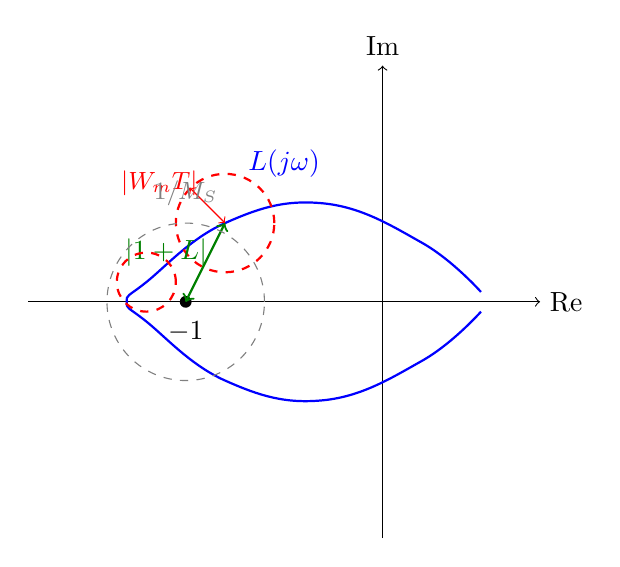
\begin{tikzpicture}[scale=2.5]
    % Axes
    \draw [->] (-1.8, 0) -- (0.8, 0) node[right] {Re};
    \draw [->] (0, -1.2) -- (0, 1.2) node[above] {Im};

    % Critical point
    \fill (-1, 0) circle (0.03);
    \node at (-1, -0.15) {$-1$};

    % Nominal Nyquist curve
    \draw [blue, thick] plot [smooth, tension=0.7] coordinates
        {(0.5, 0.05) (0.2, 0.3) (-0.3, 0.5) (-0.8, 0.4) (-1.2, 0.1)
         (-1.3, 0) (-1.2, -0.1) (-0.8, -0.4) (-0.3, -0.5) (0.2, -0.3) (0.5, -0.05)};
    \node [blue] at (-0.5, 0.7) {$L(j\omega)$};

    % Uncertainty disk at one frequency
    \draw [red, thick, dashed] (-0.8, 0.4) circle (0.25);
    \draw [red, <->] (-0.8, 0.4) -- ++(-0.18, 0.18) node[midway, above left, font=\small] {$|W_m T|$};

    % Distance to -1
    \draw [green!50!black, thick, <->] (-1, 0) -- (-0.8, 0.4);
    \node [green!50!black] at (-1.1, 0.25) {$|1+L|$};

    % Another uncertainty disk
    \draw [red, thick, dashed] (-1.2, 0.1) circle (0.15);

    % Stability circle
    \draw [gray, dashed] (-1, 0) circle (0.4);
    \node [gray, font=\small] at (-1, 0.55) {$1/M_S$};
\end{tikzpicture}
\caption{Robust stability visualization in Nyquist diagram. The dashed circles represent uncertainty at different frequencies. For robust stability, no uncertainty disk may contain the critical point $-1$. The gray circle shows the minimum distance to $-1$, equal to $1/M_S$.}
\label{fig:nyquist_robust}
\end{figure}

\subsection{Sensitivity Function Bode Plots}

\begin{figure}[htbp]
\centering
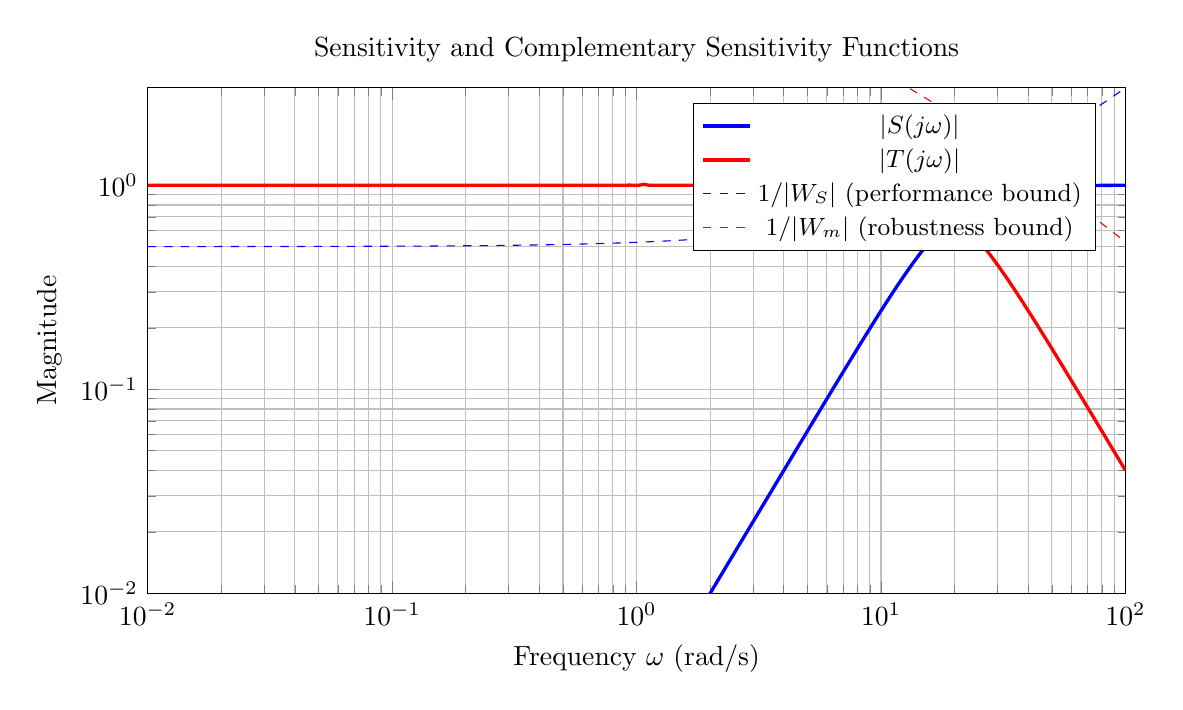
\begin{tikzpicture}
\begin{semilogyaxis}[
    width=14cm, height=8cm,
    xlabel={Frequency $\omega$ (rad/s)},
    ylabel={Magnitude},
    xmin=0.01, xmax=100,
    ymin=0.01, ymax=3,
    xmode=log,
    grid=both,
    legend pos=north east,
    legend style={font=\small},
    title={Sensitivity and Complementary Sensitivity Functions}
]

% Sensitivity function
\addplot[blue, very thick, domain=0.01:100, samples=200]
    {1/sqrt(1 + (20/x)^4)};
\addlegendentry{$|S(j\omega)|$}

% Complementary sensitivity
\addplot[red, very thick, domain=0.01:100, samples=200]
    {(20/x)^2/sqrt(1 + (20/x)^4)};
\addlegendentry{$|T(j\omega)|$}

% Inverse weights
\addplot[blue, dashed, domain=0.01:100, samples=100]
    {0.5 + 0.5*x/20};
\addlegendentry{$1/|W_S|$ (performance bound)}

\addplot[red, dashed, domain=0.01:100, samples=100]
    {1/(0.1 + 0.9*x/50)};
\addlegendentry{$1/|W_m|$ (robustness bound)}

% Peak sensitivity
\draw [<-, thick] (axis cs:8, 1.2) -- (axis cs:15, 1.8)
    node[right, font=\small] {$M_S$ (peak)};

\end{semilogyaxis}
\end{tikzpicture}
\caption{Bode plot of sensitivity functions with design bounds. The sensitivity $|S|$ should remain below $1/|W_S|$ for performance; the complementary sensitivity $|T|$ should remain below $1/|W_m|$ for robust stability. The peak sensitivity $M_S$ indicates robustness margins.}
\label{fig:sensitivity_bode}
\end{figure}

\subsection{Nominal vs Robust Response Comparison}

\begin{figure}[htbp]
\centering
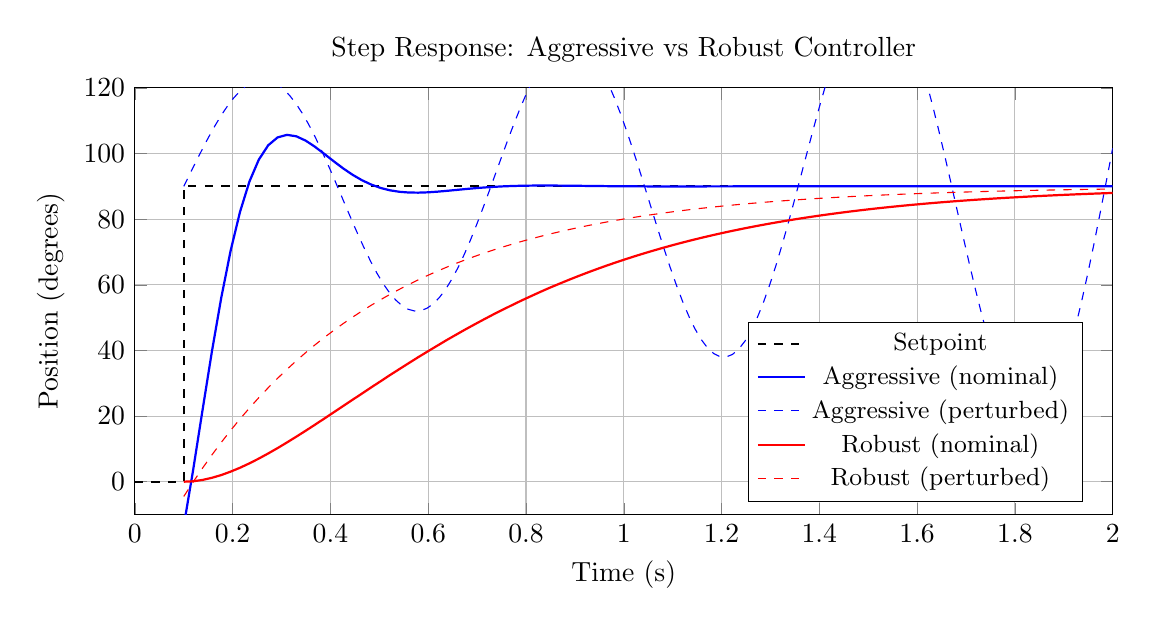
\begin{tikzpicture}
\begin{axis}[
    width=14cm, height=7cm,
    xlabel={Time (s)},
    ylabel={Position (degrees)},
    xmin=0, xmax=2,
    ymin=-10, ymax=120,
    grid=both,
    legend pos=south east,
    legend style={font=\small},
    title={Step Response: Aggressive vs Robust Controller}
]

% Setpoint
\addplot[black, thick, dashed] coordinates {(0,0) (0.1,0) (0.1,90) (2,90)};
\addlegendentry{Setpoint}

% Aggressive controller - nominal
\addplot[blue, thick, domain=0.1:2, samples=100]
    {90*(1 - 1.15*exp(-8*(x-0.1))*cos(deg(12*(x-0.1))))};
\addlegendentry{Aggressive (nominal)}

% Aggressive controller - perturbed (unstable oscillation)
\addplot[blue, dashed, domain=0.1:2, samples=150]
    {90 + 30*exp(0.5*(x-0.1))*sin(deg(10*(x-0.1)))};
\addlegendentry{Aggressive (perturbed)}

% Robust controller - nominal
\addplot[red, thick, domain=0.1:2, samples=100]
    {90*(1 - exp(-3*(x-0.1)) - 3*(x-0.1)*exp(-3*(x-0.1)))};
\addlegendentry{Robust (nominal)}

% Robust controller - perturbed
\addplot[red, dashed, domain=0.1:2, samples=100]
    {90*(1 - 1.05*exp(-2.5*(x-0.1)))};
\addlegendentry{Robust (perturbed)}

\end{axis}
\end{tikzpicture}
\caption{Comparison of step responses. The aggressive controller provides fast response at nominal conditions but becomes unstable when the plant is perturbed (e.g., increased payload inertia). The robust controller is slower but maintains stability and acceptable performance across the uncertainty range.}
\label{fig:response_comparison}
\end{figure}

%=============================================================================
\section{Chapter Summary}
\label{sec:summary}
%=============================================================================

This chapter developed the theory and practice of robust control---designing controllers that maintain stability and performance despite model uncertainty.

\begin{enumerate}
    \item \textbf{Historical Foundation}: Robust control concepts emerged from practical necessity. Bode's sensitivity analysis for telephone amplifiers, Doyle and Stein's exposure of LQG robustness problems, and Zames's $H_\infty$ framework all addressed the fundamental reality that models are never perfect.

    \item \textbf{Types of Uncertainty}: We distinguished parametric uncertainty (known structure, uncertain values), unstructured uncertainty (unknown high-frequency dynamics), and additive versus multiplicative formulations. Each type requires appropriate mathematical treatment.

    \item \textbf{Small Gain Theorem}: The cornerstone of robust stability analysis provides a frequency-domain condition: $\|W_m T\|_\infty < 1$ for multiplicative uncertainty. This elegantly connects the uncertainty bound $W_m$ to the required roll-off of complementary sensitivity $T$.

    \item \textbf{Sensitivity Trade-offs}: The identity $S + T = 1$ forces a fundamental trade-off. Low sensitivity to disturbances (small $|S|$) at one frequency range must be paid for by high complementary sensitivity (large $|T|$) elsewhere. Good design manages this trade-off explicitly.

    \item \textbf{Practical Margins}: Classical gain and phase margins remain valuable robustness indicators. The sensitivity peak $M_S$ provides a unified robustness measure with guaranteed minimum margins.

    \item \textbf{$H_\infty$ Control}: The $H_\infty$ framework transforms robust design into optimization: minimize the worst-case performance over all plants in the uncertainty set. This provides a systematic approach to robust controller synthesis.
\end{enumerate}

\begin{tcolorbox}[colback=yellow!10!white,colframe=orange!75!black,title=Key Takeaway]
All models are wrong. A controller designed only for nominal conditions will eventually fail. Robust design explicitly accounts for uncertainty, trading peak performance for reliability across a range of operating conditions. In safety-critical systems, this trade-off is not optional---it is the difference between success and catastrophe.
\end{tcolorbox}

%=============================================================================
\section{Problems}
\label{sec:problems}
%=============================================================================

\begin{enumerate}
    \item \textbf{Margins from Bode Plot}: For a system with loop transfer function $L(s) = \dfrac{50}{s(s+1)(s+10)}$, calculate the gain margin and phase margin. Assess whether the system meets typical robustness specifications.

    \item \textbf{Sensitivity Peak}: A control system has sensitivity function $S(s) = \dfrac{s^2 + 2s + 1}{s^2 + 3s + 10}$. Calculate $M_S = \|S\|_\infty$ and determine the guaranteed minimum gain and phase margins.

    \item \textbf{Multiplicative Uncertainty}: A plant has multiplicative uncertainty weight $W_m(s) = \dfrac{s+1}{s+20}$. If the complementary sensitivity at $\omega = 10$ rad/s has magnitude $|T(j10)| = 0.5$, is the robust stability condition satisfied at this frequency?

    \item \textbf{Small Gain Application}: A feedback system has $G(s) = \dfrac{2}{(s+1)^2}$ and $K(s) = 3$. An additive uncertainty $\Delta_a$ satisfies $|\Delta_a(j\omega)| \leq 0.1\omega^2$ for all $\omega$. Determine if the system is robustly stable.

    \item \textbf{Lead Compensator Design}: Design a lead compensator for $G(s) = \dfrac{5}{s(s+2)}$ to achieve phase margin $\geq 60°$ with gain crossover frequency $\omega_c = 4$ rad/s.

    \item \textbf{Parametric to Multiplicative}: A spring-mass system has uncertain stiffness $k \in [80, 120]$ N/m with nominal $k_0 = 100$ N/m and mass $m = 1$ kg. Express the plant uncertainty in multiplicative form and determine the weight $W_m(s)$.

    \item \textbf{$H_\infty$ Interpretation}: Explain the physical meaning of minimizing $\|W_S S\|_\infty$ where $W_S(s) = \dfrac{s/M + \omega_B}{s + \omega_B A}$ with $M = 2$, $\omega_B = 10$ rad/s, and $A = 0.01$.

    \item \textbf{Laboratory Analysis}: In the robust motor control experiment, a student finds that the aggressive controller becomes unstable when payload mass increases from 0g to 50g. If the nominal time constant is $\tau_0 = 0.1$ s and increases to $\tau = 0.15$ s with the 50g payload, calculate how much the phase margin at the original crossover frequency has decreased.

    \item \textbf{Monte Carlo}: Describe a procedure to assess robust performance using Monte Carlo simulation for a system with three uncertain parameters, each uniformly distributed over a $\pm 20\%$ range.

    \item \textbf{Design Trade-off}: A system requires $|S(j\omega)| < 0.1$ for $\omega < 1$ rad/s and $|T(j\omega)| < 0.1$ for $\omega > 100$ rad/s. Sketch a typical sensitivity/complementary sensitivity pair that meets these requirements and identify the crossover frequency range.
\end{enumerate}

%=============================================================================
% End of Chapter
%=============================================================================
